%%%%%%%%%%%%%%%%%%%%%%%%%%%%%%%%%%%%%%%%%
% Masters/Doctoral Thesis 
% LaTeX Template
% Version 2.5 (27/8/17)
%
% This template was downloaded from:
% http://www.LaTeXTemplates.com
%
% Version 2.x major modifications by:
% Vel (vel@latextemplates.com)
%
% This template is based on a template by:
% Steve Gunn (http://users.ecs.soton.ac.uk/srg/softwaretools/document/templates/)
% Sunil Patel (http://www.sunilpatel.co.uk/thesis-template/)
%
% Template license:
% CC BY-NC-SA 3.0 (http://creativecommons.org/licenses/by-nc-sa/3.0v/)
%
%%%%%%%%%%%%%%%%%%%%%%%%%%%%%%%%%%%%%%%%%


%----------------------------------------------------------------------------------------
%	PACKAGES AND OTHER DOCUMENT CONFIGURATIONS
%----------------------------------------------------------------------------------------

\documentclass[
%in original
11pt, % The default document font size, options: 10pt, 11pt, 12pt
%oneside, % Two side (alternating margins) for binding by default, uncomment to switch to one side
english, % ngerman for German
singlespacing, % Single line spacing, alternatives: onehalfspacing or doublespacing
%
%draft, % Uncomment to enable draft mode (no pictures, no links, overfull hboxes indicated)
%
%nolistspacing, % If the document is onehalfspacing or doublespacing, uncomment this to set spacing in lists to single
%
liststotoc, % Uncomment to add the list of figures/tables/etc to the table of contents
%toctotoc, % Uncomment to add the main table of contents to the table of contents
%parskip, % Uncomment to add space between paragraphs
%nohyperref, % Uncomment to not load the hyperref package
headsepline, % Uncomment to get a line under the header
%chapterinoneline, % Uncomment to place the chapter title next to the number on one line
%consistentlayout, % Uncomment to change the layout of the declaration, abstract and acknowledgements pages to match the default layout
]{MastersDoctoralThesis} % The class file specifying the document structure

% Required for inputting international characters
\usepackage[utf8]{inputenc}
% Output font encoding for international characters
\usepackage[T1]{fontenc}

% facilitate commenting
\usepackage{comment}

% Use the Palatino font by default
\usepackage{mathpazo}

% Use the bibtex backend with the authoryear citation style (which resembles APA)
%\usepackage[backend=bibtex,style=authoryear,natbib=true]{biblatex}

\usepackage[citestyle=authoryear,
			bibstyle=authoryear,
			natbib=true,
			backend=biber,
            maxbibnames=10,
			maxcitenames=2,
            giveninits=true,
            uniquename=init,
            terseinits = true,
            dashed=false
			]{biblatex}

% The filename of the bibliography
\addbibresource{bibliography.bib}

% Required to generate language-dependent quotes in the bibliography
\usepackage[autostyle=true]{csquotes}

% none of the packages worked as expected
\usepackage{textcomp} % to be able to use \textdegree

% package to handle units
\usepackage{siunitx}
% make a / to indicate "per"
\sisetup{per-mode=symbol}


% for prettier tables
\usepackage{booktabs} 

% use a glossary (file is still there if wanted)
%\usepackage[acronym,toc,nonumberlist]{glossaries} % use acronyms
%\makeglossaries

% to display code
\usepackage{listings}

% remove indentation
\setlength{\parindent}{0in}


%----------------------------------------------------------------------------------------
%	MARGIN SETTINGS
%----------------------------------------------------------------------------------------


% original page settings
% \geometry{
% 	paper=a4paper, % Change to letterpaper for US letter
% 	inner=2.5cm, % Inner margin
% 	outer=3.8cm, % Outer margin
% 	bindingoffset=.5cm, % Binding offset
% 	top=1.5cm, % Top margin
% 	bottom=1.5cm, % Bottom margin
% 	%showframe, % Uncomment to show how the type block is set on the page
% }

\geometry{paper= a4paper,
				left=5cm,%
                right=2cm,%
                top=2.25cm,%
                bottom=2.25cm,%
                headheight=12pt}%
   


%----------------------------------------------------------------------------------------
%	THESIS INFORMATION
%----------------------------------------------------------------------------------------

 % Your thesis title, this is used in the title and abstract, print it elsewhere with \ttitle
\thesistitle{A new eye tracking test battery: Evaluation of Pupil Labs glasses against EyeLink~1000}
%An analysis of gaze data quality of two simultaneously recorded eye trackers using a new extensive eye movement test battery}
\supervisor{Prof.\ Dr.\ med.\ Peter König} % Your supervisor's name, this is used in the title page, print it elsewhere with \supname
\examiner{Dr.\ Benedikt Ehinger} % Your examiner's name, this is not currently used anywhere in the template, print it elsewhere with \examname
\degree{Bachelor of Science} % Your degree name, this is used in the title page and abstract, print it elsewhere with \degreename
\author{Katharina Groß} % Your name, this is used in the title page and abstract, print it elsewhere with \authorname
\addresses{} % Your address, this is not currently used anywhere in the template, print it elsewhere with \addressname

\subject{Cognitive Science} % Your subject area, this is not currently used anywhere in the template, print it elsewhere with \subjectname
\keywords{Eye Tracking} % Keywords for your thesis, this is not currently used anywhere in the template, print it elsewhere with \keywordnames
\university{\href{https://www.uni-osnabrueck.de/en/home.html}{Osnabrück University}} % Your university's name and URL, this is used in the title page and abstract, print it elsewhere with \univname
\department{\href{https://www.ikw.uni-osnabrueck.de/en/home.html}{Institute of Cognitive Science}} % Your department's name and URL, this is used in the title page and abstract, print it elsewhere with \deptname
\group{\href{https://www.ikw.uni-osnabrueck.de/en/research_groups/neurobiopsychology.html}{Research Group Neurobiopsychology}} % Your research group's name and URL, this is used in the title page, print it elsewhere with \groupname
\faculty{\href{https://www.uni-osnabrueck.de/universitaet/fachbereiche/fachbereich_humanwissenschaften.html}{School of Human Sciences}} % Your faculty's name and URL, this is used in the title page and abstract, print it elsewhere with \facname


%%%%% BEGIN SECTION REDEFINITIONS
% Redefine different sections and section* to be of a higher level and
% introduce chapters, such that in the thesis the levels from the PeerJ journal
% can properly be reused.
\makeatletter

\let\oldChapter\chapter
\let\oldSection\section
\let\oldSubSection\subsection
\let\oldSubSubSection\subsubsection
\let\oldParagraph\paragraph

\def\section{\@ifstar\@section\@@section}
\def\@section#1{\oldChapter{#1}}
\def\@@section#1{\oldChapter{#1}}

\def\subsection{\@ifstar\@subsection\@@subsection}
\def\@subsection#1{\oldSection{#1}}
\def\@@subsection#1{\oldSection{#1}}

\def\subsubsection{\@ifstar\@subsubsection\@@subsubsection}
\def\@subsubsection#1{\oldSubSection{#1}}
\def\@@subsubsection#1{\oldSubSection{#1}}

\def\paragraph{\@ifstar\@paragraph\@@paragraph}
\def\@paragraph#1{\oldSubSubSection{#1}}
\def\@@paragraph#1{\oldSubSubSection{#1}}

\makeatother
%%%%% END SECTION REDEFINITIONS




\AtBeginDocument{
\hypersetup{pdftitle=\ttitle} % Set the PDF's title to your title
\hypersetup{pdfauthor=\authorname} % Set the PDF's author to your name
\hypersetup{pdfkeywords=\keywordnames} % Set the PDF's keywords to your keywords
}

\begin{document}

% Use roman page numbering style (i, ii, iii, iv...) for the pre-content pages
\frontmatter
\thispagestyle{empty}
%\pagenumbering{gobble}

\pagestyle{plain} % Default to the plain heading style until the thesis style is called for the body content


%----------------------------------------------------------------------------------------
%	TITLE PAGE
%----------------------------------------------------------------------------------------

\begin{titlepage}
	\begin{center}
		
		\vspace*{.06\textheight}
		{\scshape\LARGE \univname\par}\vspace{1.5cm} % University name
		\textsc{\Large Bachelor's Thesis}\\[0.5cm] % Thesis type
		
		\HRule \\[0.4cm] % Horizontal line
		{\huge \bfseries \ttitle\par}\vspace{0.4cm} % Thesis title
		\HRule \\[1.5cm] % Horizontal line
		 
		\begin{minipage}[t]{0.4\textwidth}
			\begin{flushleft} \large
				\emph{Author:}\\
				\href{https://www.ikw.uni-osnabrueck.de/en/research_groups/neurobiopsychology/people.html}{\authorname} % Author name - remove the \href bracket to remove the link
			\end{flushleft}
		\end{minipage}
		\begin{minipage}[t]{0.4\textwidth}
			\begin{flushright} \large
				\emph{Supervisors:} \\
				\href{https://www.ikw.uni-osnabrueck.de/en/research_groups/neurobiopsychology/people.html}{\supname} \\% Supervisor name - remove the \href bracket to remove the link 
                \href{https://www.ikw.uni-osnabrueck.de/en/research_groups/neurobiopsychology/people.html}{\examname}
			\end{flushright}
		\end{minipage}\\[3cm]
		 
		\vfill
		
		\large \textit{A thesis submitted in fulfillment of the requirements\\ for the degree of \degreename}\\[0.3cm] % University requirement text
		\textit{in the}\\[0.4cm]
		\groupname\\\deptname\\[2cm] % Research group name and department name
		 
		\vfill
		
		{\large \today}\\[4cm] % Date
		%\includegraphics{Logo} % University/department logo - uncomment to place it
		 
		\vfill
	\end{center}
\end{titlepage}


%----------------------------------------------------------------------------------------
%	ABSTRACT PAGE
%----------------------------------------------------------------------------------------

\begin{abstract}
	%\addchaptertocentry{\abstractname} % Add the abstract to the table of contents
	
    % add content of Abstract tex file here
	Eye tracking experiments rely heavily on good data quality of eye trackers. 
Unfortunately, often only spatial accuracy and precision values are available from the manufacturers.
These two values alone are not sufficient to reasonably benchmark an eye tracker:
The values will deteriorate drastically during an experimental session due to head movements, changing illumination or calibration decay in general. In addition, different experimental paradigms allow to analyze different types of eye movements which cannot be evaluated by spatial accuracy or precision, for instance smooth pursuit movements, blinks or microsaccades.
To obtain a more comprehensive description of properties, we developed an extensive eye tracking test battery.
In 10 different tasks, we evaluated eye tracking related measures such as: the decay of accuracy, pupil dilation, smooth pursuit movement, microsaccade detection, blink detection, and the influence of head motion.
For some measures true theoretical values exist, for others, a relative comparison to a gold standard eye tracker is needed.
Therefore, we collected our gaze data simultaneously from a gold standard remote EyeLink~1000 (\SI{500}{\hertz}) eye tracker and the mobile Pupil Labs glasses (\SI{120}{\hertz} -- \SI{240}{\hertz}).

\end{abstract}


%----------------------------------------------------------------------------------------
%	ACKNOWLEDGEMENTS
%----------------------------------------------------------------------------------------

%\begin{acknowledgements}
%\end{acknowledgements}


%----------------------------------------------------------------------------------------
%	LIST OF CONTENTS/FIGURES/TABLES PAGES
%----------------------------------------------------------------------------------------

\tableofcontents % Prints the main table of contents

%----------------------------------------------------------------------------------------
%	THESIS CONTENT - CHAPTERS
%----------------------------------------------------------------------------------------

% Begin numeric (1,2,3...) page numbering
\mainmatter 
%\pagenumbering{arabic}

% Return the page headers back to the "thesis" style
\pagestyle{thesis}

% Include the chapters of the thesis as separate files from the Chapters folder

%----------------------------------------------------------------------------------------
%	INTRODUCTION
%----------------------------------------------------------------------------------------
\section{Introduction}

TODO: Introduction to the project and motivation behind it.

\subsection{The project}

TODO: Rough summary of the idea of the project.
How did the idea come up?
What is the project about?

\subsection{Background on computer vision based classification tasks}

TODO: Short introduction into the fields of machine learning, computer vision, and to artificial neural networks. Prospects and challenges of both on a general basis with respect to our issue. This part is kept brief.

\subsection{Background on sorting asparagus}

\begin{figure}[h]
	\centering
	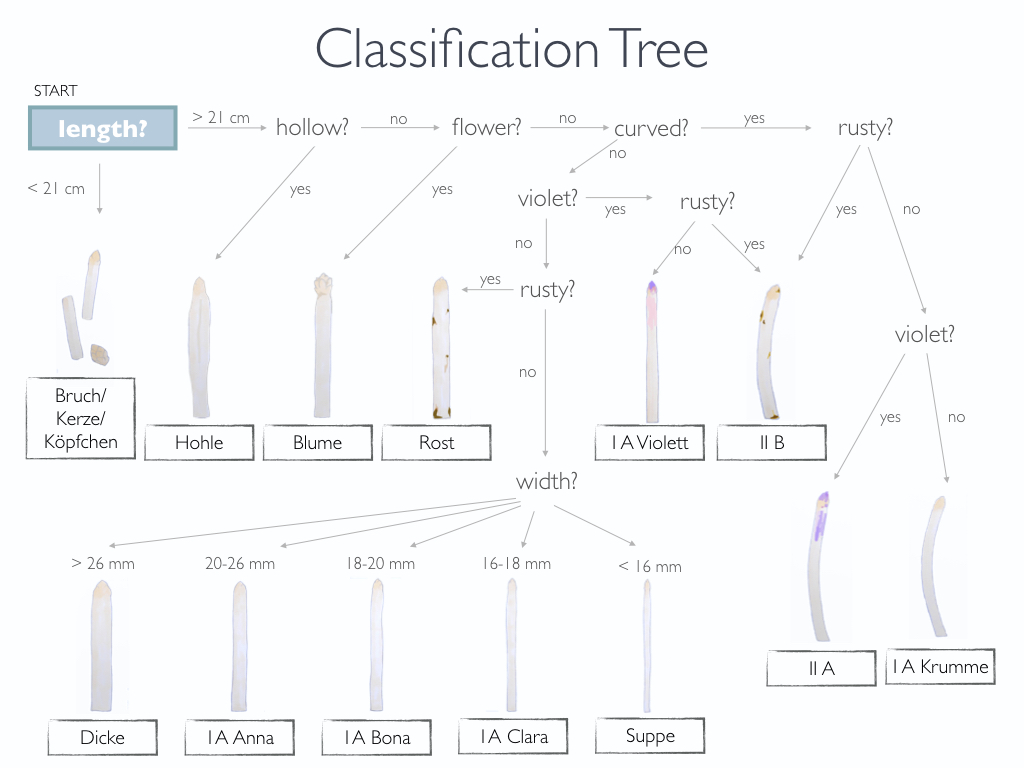
\includegraphics[scale=0.35]{Figures/chapter01/fig_tree_with_title}
	\decoRule
	\caption[Decision tree for labels]{The decision tree for attributing a label to the asparagus as to the sorting rules of the asparagus farm "Gut Holsterfeld". Starting from the upper left corner of the image binary decisions are made until a label is reached (except for Width).}
	\label{fig:LabelTree}
\end{figure}

TODO: What is the main focus during the sorting process, i.e. why do you need to sort asparagus and in which classes do you sort it? \\
What problems and challenges will be met - including the difference of challenge for humans vs. machines. \\
Including the description of the labels as sorted by Hof Gut Holsterfeld (Figure~\ref{fig:LabelTree}).


\subsection{Expected outcome vs. actual outcome of the project}

Based on the literature review, we aimed to improve the current sorting performance of the XX machine at the local asparagus farm “Spargelhof Gut Holsterfeld”. In this report, we investigated techniques from computer vision, both classical and deep learning based approaches. We expected to reach a result which is able to classify asparagus images into 13 different classes better than the current standard. For the initial performance of the sorting machine, no reliable accuracy of correctly sorted asparagus pieces is available, but between three and six workers are employed to re-sort wrongly classified asparagus pieces. The farmer himself assumes an accuracy of not more than 70\%. \\
 
An advantage of our project is that it was directly supported by the local asparagus farm, providing training data and allowing us to evaluate our proposed solutions in a real environment during the asparagus harvesting season 2020. \\
\\
However, there was a misunderstanding between us and the supporting asparagus farm about the kind of data we need. The existing images were too few, and also unlabelled. Therefore, we spent the first two and a half months with data acquisition instead of starting with preprocessing as we originally planned. Throughout the harvesting season 2019, we continuously went to the asparagus farm and collected unlabelled asparagus images during the normal harvesting procedure. For a small amount of asparagus pieces (xx in total), we collected labelled data by taking images of pre-sorted asparagus pieces. Pre-sorted in this context means that the asparagus pieces were sorted by the sorting machine and if needed re-sorted manually by professional workers. \\
The number of labelled images is insufficient to learn classes using deep learning approaches~\citep{russakovsky2013detecting} ~\citep{russakovsky2010attribute} (\url{https://petewarden.com/2017/12/14/how-many-images-do-you-need-to-train-a-neural-network/}). Therefore, we spent six months preprocessing and labelling the data manually. Preprocessing involved: organizing the large number of images, renaming the files, so that the three images of one asparagus piece can be accessed together, and performing automatic feature extractions (ref to preprocessing).To label the images by hand, we wrote a custom application (reference hand-label-assistant). The final labelled data set contains over 10.000 (genaue Zahl an stangen) labelled asparagus pieces. Next, we worked on numerous classical and deep learning approaches (ref to chap 4). We reached several very interesting results which will be discussed in Chapter 4. Although we developed an end-to-end prototype, we did not deploy it onto the sorting machine for the harvesting season 2020. Even though some of our results are highly promising, it is therefore difficult to compare it to the current performance of the machine. \\
 \\
Hier noch ein Absatz mit den Inhalten aus der Conclusion – sobald diese steht. 





%----------------------------------------------------------------------------------------
%	THESIS CONTENT - APPENDICES
%----------------------------------------------------------------------------------------
\appendix % Cue to tell LaTeX that the following "chapters" are Appendices

% Include the appendices of the thesis as separate files from the Appendices folder
% \include{Appendices/AppendixCommentSheet}

%----------------------------------------------------------------------------------------
%	BIBLIOGRAPHY
%----------------------------------------------------------------------------------------

\printbibliography[heading=bibintoc]




%----------------------------------------------------------------------------------------

\end{document}  
